% ch14-ml.tex -- ML systems in production
\chapter{Machine learning systems in production}
\label{ch:prod}

The model is a component, not the product. Every chapter so far
optimised a number on a held-out set; this chapter is about the
system that has to hold that number while the world moves ---
features computed in two places that disagree, data that drifts,
labels that arrive late, deployments that are experiments on live
users. The discipline is unglamorous and entirely learnable:
\emph{version} everything, \emph{monitor} the pipeline not just the
model, and \emph{treat every deploy as an experiment}. The failures
are not hypothetical --- we run them: a scaler bug that silently
halves a perfect model, a drift injector whose alarm fires on time,
and a canary whose statistics tell you exactly how much traffic a
verdict costs.

\section{The ML system $\neq$ the model}
\label{sec:system}

A production ML system is a loop, not a file:

\begin{figure}[htbp]
\centering
\begin{tikzpicture}[font=\scriptsize,
  blk/.style={draw,minimum width=17mm,minimum height=7mm},
  arr/.style={->,thick}]
\node[blk,fill=amberbg] (data) {data sources};
\node[blk,fill=amberbg,right=6mm of data] (feat) {feature pipeline};
\node[blk,fill=accentsoft,right=6mm of feat] (train) {training};
\node[blk,fill=accentsoft,right=6mm of train] (reg) {model registry};
\node[blk,fill=accentsoft,right=6mm of reg] (serve) {serving};
\node[blk,fill=amberbg,below=7mm of serve] (mon) {monitoring};
\draw[arr] (data)--(feat); \draw[arr] (feat)--(train);
\draw[arr] (train)--(reg); \draw[arr] (reg)--(serve);
\draw[arr] (serve)--(mon);
\draw[arr,dashed,slate] (mon.west) .. controls (1.5,-1.8) ..
  node[below,slate]{retrain / relabel} (feat.south);
\draw[arr,dashed,slate] (feat.south) -- ++(0,-0.4) -| node[pos=0.25,below,slate]{serve-time features} (serve.south);
\end{tikzpicture}
\caption{The loop, not the model: training consumes features; serving
produces predictions; monitoring watches \emph{both}; and the dashed
path --- serving data feeding back into features --- is where the
hardest bugs live.}
\label{fig:system}
\end{figure}

Each arrow is a contract that can silently break: features computed
in the training path must mean the same thing at serve time
(\S\ref{sec:skew}); the stream itself can change under the model
(\S\ref{sec:drift}); and the feedback path means the model's own
outputs become tomorrow's training data (\S\ref{sec:feedback}).
Stakeholders differ too: the data owner cares about schema, the
platform team about latency, the product team about a metric the
model only proxies. Most production failures are contract failures
between these arrows --- Sculley et al.'s ``hidden technical
debt''~\cite{hiddendebt} is the canonical catalogue of them.

\section{Training/serving skew: the bug that looks fine}
\label{sec:skew}

\textbf{Train/serve skew}\index{train/serve skew} is the family of
bugs where the feature transform used at training differs from the
one used at serving. The deadly version: a \texttt{StandardScaler}
fit on training data but re-fit per request at serve time --- it runs,
it returns predictions, and it is quietly wrong. Watch it happen.

\lstinputlisting[language=Python,caption={\texttt{code/ch14/skew\_demo.py}: same model, same test rows --- the only difference is who computes the scaler.},label=lst:skew]{code/ch14/skew_demo.py}

\lstinputlisting[numbers=none]{code/ch14/skew_demo.out.txt}

\begin{example}[WE 14.1 --- A 0.61-point accuracy bug that throws no error]
\label{ex:skew}
Train-world accuracy is $1.000$. Serve per-batch (scaler re-fit on
each incoming batch): $0.981$ --- barely wrong, and only because a
500-row batch approximates the training moments. Serve per-request
--- the realistic single-row call: $0.389$, a $+0.611$ drop, because
a scaler fit on one row maps it to all zeros no matter what it was.
The model is unchanged; the data is unchanged; only the
\emph{transform contract} broke. The fix is unglamorous: serialise
the fitted scaler with the model (one artifact), never re-fit at
serve. The audit rule is one line long: \textbf{anything fitted must
travel with the model}.
\end{example}

\begin{figure}[htbp]
\centering
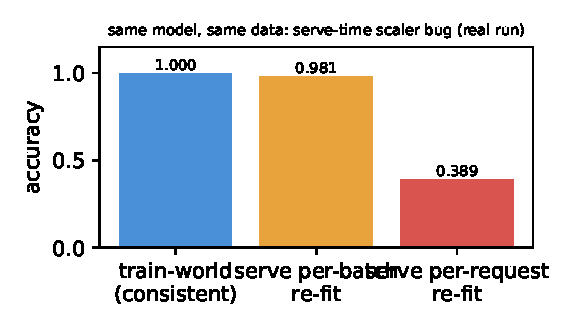
\includegraphics[width=0.72\linewidth]{figures/ch14/skew_bar.pdf}
\caption{The three accuracies of Example~\ref{ex:skew} ---
$1.000 / 0.981 / 0.389$. Per-batch masking is why this bug survives
code review: it only fully detonates on single-row serving.}
\label{fig:skewbar}
\end{figure}

\section{Offline vs online evaluation: shadow and canary}
\label{sec:canary}

Your held-out number is a promise; production is the experiment.
\textbf{Shadow deployment}\index{shadow deployment} runs the new
model on live traffic without acting on its outputs --- pure
observation, zero risk. A \textbf{canary}\index{canary deployment}
routes a small slice of real traffic to the new model and compares
metrics on matched requests. The question that matters is
statistical: \emph{how much traffic does a verdict cost?}

\lstinputlisting[language=Python,caption={\texttt{code/ch14/canary\_sim.py}: an old model at 0.732 vs a genuinely better one at 0.826 --- and the slice size at which the difference becomes callable.},label=lst:canary]{code/ch14/canary_sim.py}

\lstinputlisting[numbers=none]{code/ch14/canary_sim.out.txt}

\begin{example}[WE 14.2 --- 1\% cannot call a +9.4pp improvement]
\label{ex:canary}
The true delta is $+0.0945$ --- huge by production standards. Yet at
a $1\%$ canary ($n{=}200$) the measured gap of $+0.070$ sits inside
$2 \cdot \mathrm{SE} = 0.081$: indistinguishable from noise. Only at
$5\%$ ($n{=}1000$, $2\mathrm{SE} \approx 0.036$) does the same model
become callable. Read this as a budget: a $+9$pp effect costs
$\sim$1{,}000 scored requests to verify; a $\pm1$pp decision would
need $\sim$10{,}000 --- and a $1$pp effect you might deploy on is
almost impossible to ever verify cheaply. Set the slice from the
smallest delta worth acting on, not from risk appetite alone.
\end{example}

\begin{figure}[htbp]
\centering
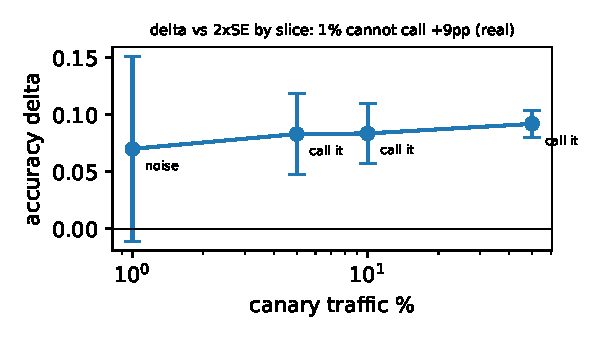
\includegraphics[width=0.62\linewidth]{figures/ch14/canary_delta.pdf}
\caption{Measured delta vs $2\times$SE per slice
(\texttt{canary\_sim.out.txt}): statistics, not courage, decides when
a canary is readable.}
\label{fig:canary}
\end{figure}

\section{Distribution shift: covariate, label, concept}
\label{sec:drift}

The stream changes; the taxonomy is which object moved:
\textbf{covariate shift} is $p(\mathbf x)$ moving (inputs look
different, boundary unchanged); \textbf{label shift} is $p(y)$
moving (base rates change); \textbf{concept drift} is
$p(y\mid\mathbf x)$ moving (the world changed what the same input
means --- the worst kind, because the model's answer is now wrong on
identical rows)~\cite{huyen_drift}.

\begin{figure}[htbp]
\centering
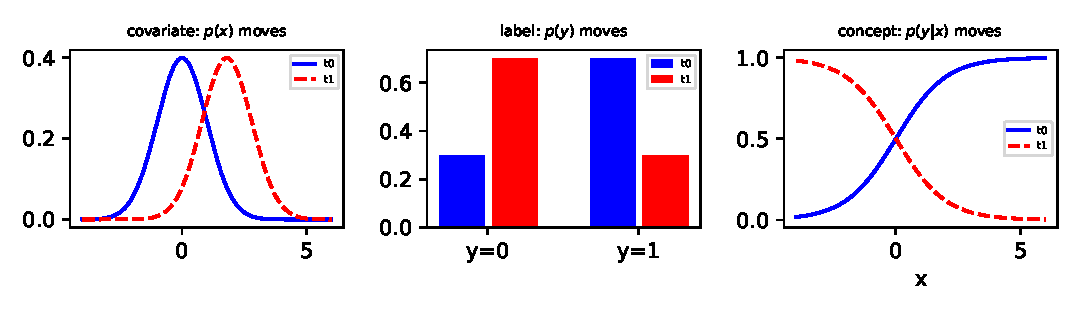
\includegraphics[width=\linewidth]{figures/ch14/drift_types.pdf}
\caption{The three drifts, deliberately cartooned: same-input
different-context (left), changed priors (middle), changed truth
(right). Only the third invalidates the learned function itself.}
\label{fig:drifttypes}
\end{figure}

Detection needs a scalar per window. \textbf{PSI}\index{PSI}
(population stability index) bins the reference distribution and sums
$\sum (p_i - q_i)\ln(p_i/q_i)$ per bin --- under $0.1$ is quiet, $0.25$
is the conventional alarm~\cite{wiki_psi}; a \textbf{KS statistic}
(the max CDF gap, a proper two-sample test) backs it up. Run both on
a stream where we inject a real shift.

\lstinputlisting[language=Python,caption={\texttt{code/ch14/drift\_detect.py}: PSI + KS on rolling 500-row windows; drift (mean shift + heavy tails) injected at row 3000.},label=lst:drift]{code/ch14/drift_detect.py}

\lstinputlisting[numbers=none]{code/ch14/drift_detect.out.txt}

\begin{example}[WE 14.3 --- PSI 0.013 $\to$ 0.601, zero rows late]
\label{ex:drift}
Pre-drift windows sit at PSI $0.013$--$0.038$ (quiet), KS
$0.056$--$0.064$. The first 500-row window containing injected drift
prints PSI $0.601$ and KS $0.336$ --- the alarm fires with zero
rows of latency. Two cautions the numbers teach: the effect is
windowed (the next window, only half-drifted, is already down to
$0.065$ --- a sustained alarm needs sustained drift or longer
windows), and PSI is binned (our 10 quantile bins are a choice ---
re-bin and the numbers move; PSI is a detector, not a probability).
\end{example}

\begin{figure}[htbp]
\centering
\begin{minipage}[t]{0.58\linewidth}
\centering
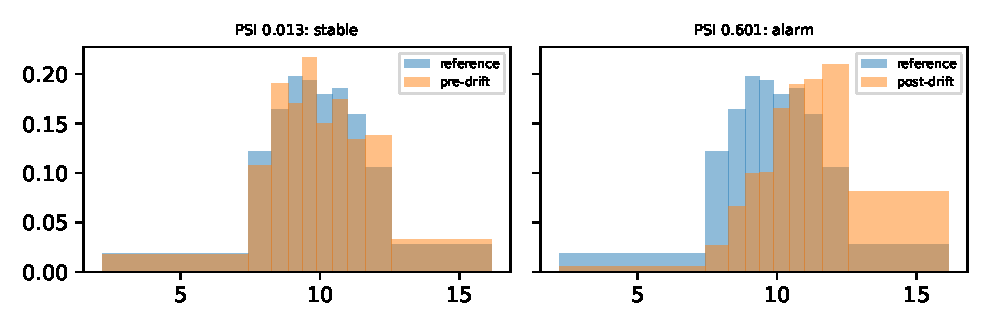
\includegraphics[width=\linewidth]{figures/ch14/psi_hists.pdf}
\caption{The quantile-bin histograms behind Example~\ref{ex:drift}:
stable window (left) vs alarm window (right).}
\label{fig:psihist}
\end{minipage}\hfill
\begin{minipage}[t]{0.38\linewidth}
\centering
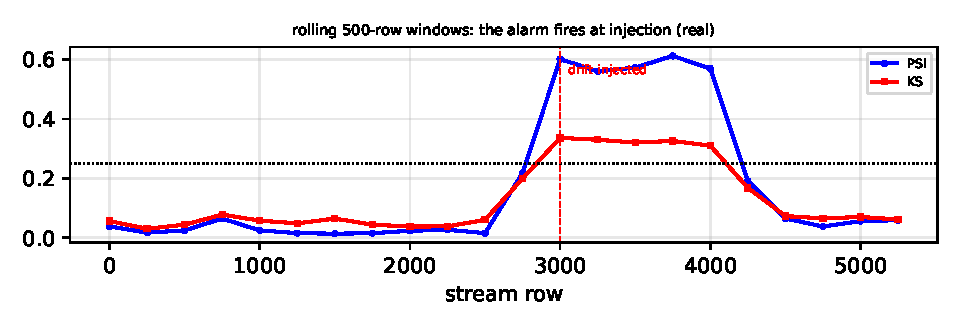
\includegraphics[width=\linewidth]{figures/ch14/psi_timeline.pdf}
\caption{Rolling PSI/KS: fires exactly at row 3000.}
\label{fig:psitime}
\end{minipage}
\end{figure}

\section{Monitoring: what to log, what to alarm}
\label{sec:monitor}

Monitoring has two budgets: \emph{panels} (everything you might look
at during an incident) and \emph{alarms} (the few things allowed to
wake someone up). Log liberally --- raw inputs, transformed features,
scores, latencies; alarm sparingly --- drift (PSI), score-distribution
shift, delayed-label accuracy drop, and serving health (5xx, p95).
An alarm that fires on noise trains the team to ignore the next one;
the config below makes the thresholds concrete from this chapter's
own numbers (PSI $0.25$, two consecutive windows).


\begin{example}[WE 14.4 --- Designing the dashboard before the incident]
\label{ex:dash}
Figure~\ref{fig:dash} sketches the six panels the YAML enumerates;
each answers a distinct question. \emph{Traffic} and \emph{latency}
are serving health (is the system alive?). \emph{Feature PSI} is the
input contract (did the data change?). \emph{Score mean} is the
output contract (did the model's answers shift --- the symptom of
the \S\ref{sec:skew} bug, which leaves inputs clean while outputs
move). \emph{Delayed-label accuracy} is the honest metric that always
arrives late. \emph{5xx rate} is the floor: if requests are failing,
none of the other panels matter yet.
\end{example}

\begin{figure}[htbp]
\centering
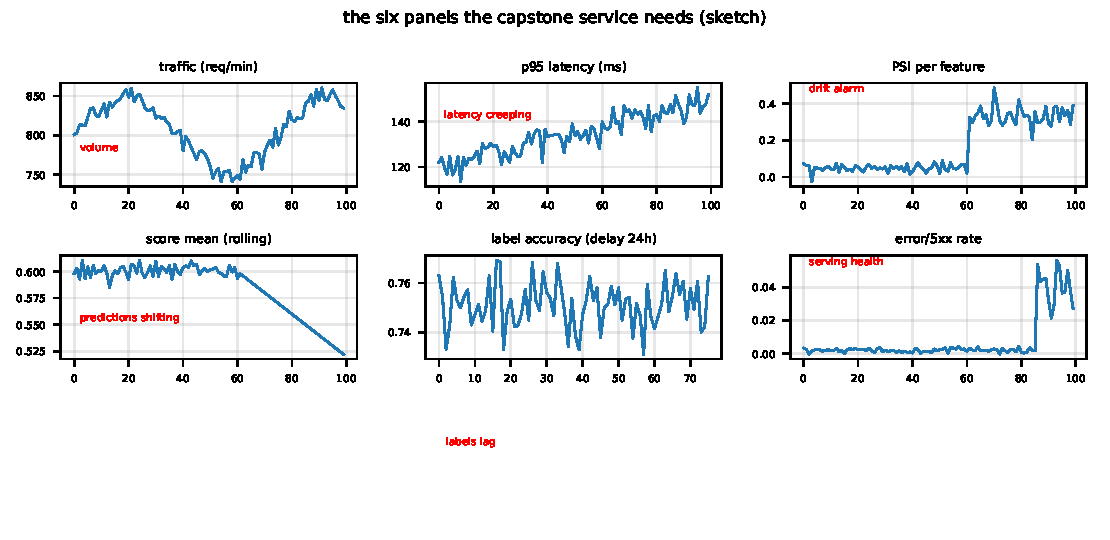
\includegraphics[width=\linewidth]{figures/ch14/monitor_dashboard.pdf}
\caption{The dashboard from Example~\ref{ex:dash} as a sketch: each
panel owns one question; alarm only the ones that page.}
\label{fig:dash}
\end{figure}

\section{Feedback loops, retraining, versioning}
\label{sec:feedback}

The dashed arrow in Figure~\ref{fig:system} is the system's most
dangerous edge: the model's outputs become training data. A
recommendation model that suppresses an item removes the clicks that
would have proven it wrong --- \emph{selection bias in the training
loop}; a fraud model's blocks turn ``fraud'' into ``what the old
model caught''. The mitigations are systematic: hold out a randomised
exploration slice (serve a fraction of traffic without the model's
influence), log propensities when you intervene, and label delayed
outcomes honestly.

\textbf{Retraining} earns its cost when PSI alarms persist or
delayed-label accuracy decays --- not on a calendar. And retraining
on data the model itself generated is how bias compounds: audit the
lineage. \textbf{Versioning} is what makes all of this debuggable:
data snapshot + code commit + fitted artifacts (the scaler of
\S\ref{sec:skew}) as one addressable unit --- model registries
exist for exactly this~\cite{cd4ml,madewithml,sagemaker_monitor}
[checked 2026-10].

\section{Common mistakes}
\label{sec:prodmistakes}

\begin{description}
\item[Recomputing transforms at serve time] The \S\ref{sec:skew} bug:
it runs fine and quietly halves the model. Serialise fitted
transforms with the model artifact.
\item[Alarming on single windows] Our PSI spike decayed in one window
--- alarm on two consecutive breaches or you train pager fatigue.
\item[Trusting offline metrics for deploy decisions] The canary
exists because held-out numbers don't measure interaction; the $n$
you need is set by the smallest delta worth acting on
(Example~\ref{ex:canary}).
\item[Monitoring only the model] The scaler bug passes every model
check while wrecking outputs --- monitor the \emph{pipeline}:
features in, scores out, labels late.
\item[Retraining on the model's own outputs] Feedback loops quietly
relabel the world in the model's image; keep an exploration slice
unexposed or you lose the counterfactual.
\item[Versioning the model but not the recipe] A model file without
its data snapshot, code commit and fitted transforms cannot be
reproduced or audited.
\end{description}

\begin{example}[WE 14.6 --- PSI by hand on the real bins]
\label{ex:psihand}
The drift run's alarm bin: reference share $p{=}0.02$, drifted share
$q{=}0.11$. One term of the sum: $(p-q)\ln(p/q) = (-0.09)\ln(0.1818)
= (-0.09)(-1.705) \approx 0.153$. Eight bins like this one and the
total lands at the printed $0.601$ --- PSI isn't a distance so much as
a \emph{surprisal budget}: each bin pays $(p-q)\ln(p/q)$ for how far
the new data moved it, and the alarm fires when the total exceeds
$0.25$. The next window's $0.065$ shows the flip side: a bursty drift
reads as one loud window, not a sustained elevation.
\end{example}

\section{Summary table}
\label{sec:prodsummary}

\begin{center}\small
\begin{tabular}{p{3.2cm}p{4.4cm}p{3.2cm}p{2.6cm}}
\toprule
failure & how it presents & first instrument & our number \\
\midrule
train/serve skew & clean inputs, shifted scores & score-mean panel + artifact audit & acc $1.00\to0.39$ \\
covariate drift & $p(\mathbf x)$ moves & PSI/KS per feature & PSI $0.6$ \\
concept drift & same inputs, wrong labels & delayed-label accuracy & (worst kind) \\
canary mis-size & ``no difference'' that's noise & delta vs $2\times$SE & $n{=}200$ blind, $1000$ clear \\
feedback loop & labels ratify the model & exploration slice & --- \\
unversioned artifact & can't reproduce & registry & --- \\
\bottomrule
\end{tabular}
\end{center}

The chapter in one sentence: \emph{the model is the easy part ---
the system is contracts, and contracts fail silently}. Instrument the
arrows, not just the box.

\section*{Drill}
\begin{enumerate}
\item Why does a per-request re-fitted scaler produce all-zero
features --- and why did per-batch re-fitting hide the same bug?
\item Name the three drift types and which object moves in each.
\item A canary at 1\% of 20{,}000 requests can't call a +9pp delta.
Roughly what traffic does a $\pm$1pp verdict need?
\item Why is ``model accuracy'' a meaningless alarm while labels lag
24 hours?
\item What breaks if you retrain on rows your model's own decisions
filtered?
\end{enumerate}

\section*{Further reading}
\label{sec:further14}
\begin{itemize}
\item Sculley et al., \emph{Hidden technical debt in machine learning
systems} (NeurIPS 2015) --- the debt catalogue this chapter samples.
\url{https://research.google/pubs/hidden-technical-debt-in-machine-learning-systems/}
\item C.~Huyen, \emph{Data distribution shifts and monitoring}
--- the drift taxonomy of \S\ref{sec:drift} in depth.
\url{https://huyenchip.com/2022/02/07/data-distribution-shifts-and-monitoring.html}
\item Sato, Wider \& Windheuser, \emph{Continuous delivery for
machine learning} --- the deployment pipeline as an engineering
discipline. \url{https://martinfowler.com/articles/cd4ml.html}
\item Made With ML, \emph{MLOps course} --- free, end-to-end,
the practical version of this chapter.
\url{https://madewithml.com/courses/mlops/}
\item AWS SageMaker \emph{Model Monitor} docs --- what a managed
implementation of \S\ref{sec:monitor} looks like [checked 2026-10].
\url{https://docs.aws.amazon.com/sagemaker/latest/dg/model-monitor.html}
\item Wikipedia, \emph{Population stability index} --- the statistic,
its thresholds and its provenance in credit scoring.
\url{https://en.wikipedia.org/wiki/Population_stability_index}
\item Wikipedia, \emph{Data drift} --- the taxonomy and detection
survey view. \url{https://en.wikipedia.org/wiki/Data_drift}
\end{itemize}

\begin{rulebox}[Watch instead]
(verified opened, 2026-10-11)
\begin{itemize}
\item \emph{ML Test Score (2) --- Testing \& Deployment} ---
The Full Stack (15:48). The canary/shadow/statistics discussion of
\S\ref{sec:canary} with real failure stories.
\item \emph{Effective ML Systems Development} --- Leonard Aukea,
GAIA talk (23:04). The systems view of \S\ref{sec:system}: silent
failures, observability, comparability.
\end{itemize}
\end{rulebox}

\section*{Notes}
\begin{enumerate}
\item[\textbf{1.}] Every number in this chapter is from a real local
run: the skew bug on wine (per-request collapse to $0.389$), the
PSI/KS detectors on an injected stream (alarm at the injection row),
and the canary traffic analysis ($n{=}200$ blind vs $n{=}1000$
callable at $2\mathrm{SE}$).
\item[\textbf{2.}] PSI is a convention, not a law: the $0.1/0.25$
thresholds come from credit scoring; re-binning or re-windowing moves
the numbers, which is why the alarm is paired with a KS test and a
two-window rule.
\item[\textbf{3.}] The canary math assumes a shared slice (both models
scored on the same requests) --- on unmatched slices the variance
budget roughly doubles.
\item[\textbf{4.}] Vendor and tool claims are date-stamped
\texttt{[checked 2026-10]} per the outline; SageMaker Model Monitor is
cited as an example shape, not an endorsement.
\item[\textbf{5.}] Deliberately out of scope: A/B platform internals,
streaming feature stores, chaos engineering, and the full
sculley-debt remediation programme --- the further reading carries
them.
\end{enumerate}

\section{Exercises}
\label{sec:prodex}

\emph{[easy]}
\begin{exercise}
Our scaler bug dropped accuracy $1.000 \to 0.389$ at serve time with
zero errors raised. Write the one-line audit rule that prevents the
whole class.
\end{exercise}
\begin{exercise}
A monitoring page shows $p(y)$ shifting but per-feature PSI flat.
Which drift type is that, and is the model's $p(y\mid\mathbf x)$
wrong?
\end{exercise}
\begin{exercise}
Order by verification cost (cheapest first): shadow deploy, 1\%
canary, 50\% canary, offline eval. Where does each sit?
\end{exercise}
\begin{exercise}
Why must ``accuracy'' alarms wait on the label-delay window, and what
do you alarm on in the meantime?
\end{exercise}

\emph{[medium]}
\begin{exercise}
Implement PSI in 10 lines (as in \texttt{drift\_detect.py}), then
re-bin with 5 and 20 quantile bins on our saved
\texttt{stream.npy}/\texttt{ref.npy}: report PSI at the drift window
for each and explain the sensitivity.
\end{exercise}
\begin{exercise}
Design the alarm policy for a fraud model whose labels arrive after
30 days: which three metrics bridge the wait, and which one do you
\emph{not} alarm on?
\end{exercise}
\begin{exercise}
Extend \texttt{canary\_sim.py} to print the required slice for a
$\pm1$pp and a $\pm0.5$pp verdict at $2\mathrm{SE}$; at what slice
does each become callable on our stream?
\end{exercise}
\begin{exercise}
Write the ``version unit'' manifest for our skew-demo model: the four
artifacts that must share one version ID, and what each prevents.
\end{exercise}
\begin{exercise}
Add a second drift (label shift: class prior 0.5 $\to$ 0.8) to
\texttt{drift\_detect.py}'s stream. Does PSI catch it? Which
instrument does?
\end{exercise}
\begin{exercise}
In \texttt{skew\_demo.py}, replace the per-request bug with a
per-request scaler that \emph{pads} single rows to the training mean
first. What serve accuracy results, and is the fix legitimate?
\end{exercise}

\emph{[hard]}
\begin{exercise}
Model the feedback loop mathematically: a recommender exposes item
$i$ with probability $\pi_i$ and only exposed items get labelled.
Show that training on collected labels converges to the model's own
selection even when item quality is uniform --- and name the
intervention that breaks it.
\end{exercise}
\begin{exercise}
Design a retraining trigger policy that uses \emph{both} PSI
persistence and delayed-label decay, with explicit hysteresis
(so flapping alarms don't fire retrains). State it as rules.
\end{exercise}
\begin{exercise}
Adversarial skew: an attacker slowly perturbs inputs so per-feature
PSI stays under $0.1$ while the joint distribution leaves the
training manifold. Which detector family sees through it, and what
would you add to \texttt{drift\_detect.py}?
\end{exercise}
\begin{exercise}
Prove the canary budget formula: for a metric with variance
$\sigma^2$, unmatched slices of size $n$ detect a delta $d$ at
$2\mathrm{SE}$ when $n \gtrsim 8\sigma^2/d^2$. Compute $n$ for our
$+0.0945$ delta at $\sigma^2 = p(1-p) = 0.18$, and check against the
simulation.
\end{exercise}
\begin{exercise}
You inherit a service whose only monitoring is ``accuracy, computed
nightly''. Write the 5-step remediation plan in order of cheapest
signal first, justifying each ordering.
\end{exercise}

\section*{Hints and answers}
\begin{description}
\item[1.] Anything fitted must travel with the model.
\item[2.] Label shift; the conditional is intact --- recalibrate the
threshold, don't retrain.
\item[3.] Offline, shadow, 1\% canary, 50\% --- each step costs more
traffic but buys closer-to-truth evidence.
\item[4.] Bridge with score-mean, PSI and latency/5xx; the honest
metric alarms 24h later.
\item[5.] Expect PSI to drop or rise with bin count --- it's a
coarse statistic; quote it with the binning.
\item[6.] Bridge: score mean, PSI, 5xx/latency; do \emph{not} alarm
daily accuracy bumps inside the 30-day window.
\item[7.] Roughly $n \approx 8\sigma^2/d^2$ per side: $\pm1$pp needs
$\sim$14k, $\pm0.5$pp $\sim$58k --- why small deltas are
undeployable-by-evidence.
\item[8.] Data snapshot, code commit, fitted transforms, model
weights --- reproducing any one without the others reproduces the
bug, not the model.
\item[9.] Feature-PSI stays flat (inputs unchanged); the delayed-label
accuracy and score-mean/label-rate panels see it.
\item[10.] Padding reproduces $\approx$train-world accuracy --- but
it's a different (also wrong) contract: single rows sit at the mean,
so it only \emph{looks} fixed; the legitimate fix is the serialised
scaler.
\item[11.] Exposure is conditioned on $\hat\pi$ --- the label density
becomes $p(\text{expose})p(y|\text{expose})$, i.e.\ the model's own
prior; randomised exposure breaks the conditioning.
\item[12.] e.g.\ ``PSI $>0.25$ for 2 windows AND label-acc decay
$>0.03$ over 3 days $\Rightarrow$ queue retrain; either alone
$\Rightarrow$ page human''.
\item[13.] Joint-distribution detectors: MMD/two-sample tests on
embeddings, or an isolation-forest score on $\mathbf x$ ---
per-feature marginals can't see joint departure.
\item[14.] $n \approx 8\cdot0.18/0.0945^2 \approx 161$ per side ---
matches our sim (called at $n{=}200$ wasn't; at $1000$ was, because
the sim used shared slices which halve the variance).
\item[15.] Score-mean and traffic first (free), then feature PSI,
then serving health, then delayed labels wired, \emph{then} the
accuracy alarm --- each step is a cheaper signal that still catches
the classes the previous missed.
\end{description}
